
\chapter{绪论}
\label{chap:introduction}

\section{论文研究背景}
\label{s:background}
当时间步入二十一世纪,互联网技术得到了飞速的发展。越来越多的人通过互联网阅读新
闻,查看邮件,分享照片。但是随着互联网的发展、数据量的飞速提升,隐私、信息的安
全保护受到了严峻的挑战。2010年以来,CSDN密码泄露事件、如家酒店开房信息泄露事件、
``棱镜门''事件等诸多信息安全事件让网络信息隐私安全受到越来越多的关注。而信息安
全学科也受到了越来越多人的重视。信息安全是一门研究信息的机密性、完整性、可用性、
可控性和不可否认性的综合学科。信息安全指出,任何系统的任何一个环节都应该得到足
够的重视,一个完备的安全保障体系是保护隐私信息的基础,它通常包括操作系统安全、
网络协议安全、管理制度安全等等。
\par
信息隐藏技术是信息安全领域下一个重要的研究方向。针对信息安全的不同属性,信息隐
藏领域又可以分为不同的方向。狭义的信息隐藏技术,也是传统意义上的信息隐藏技术,
被称为隐写术(Steganography)。隐写术是一种将秘密消息隐藏在一些公开传输的媒介中
,利用公开媒介掩护消息传输的技术,主要关注通信的隐蔽性。隐写术要求对载体进行微
量的随机修改,以防止被隐藏的消息被通信对端以外的第三方发现。与隐写术相对的技术
称为隐写分析技术(Steganalysis)。它通过对公开传输媒介的统计特征进行分析,以判
断这些媒介中是否被隐藏了消息、隐藏了怎样的消息。对隐写术、隐写分析技术的深入研
究,有助于对非法活动进行监控,对维护社会稳定,保护国家及人民安全有着至关重要的
作用。
\par
由于常规的信息隐藏技术并不关心对载体的保护,当秘密消息被提取后,载体通常不能被
完美地恢复。而这种情况在一些应用中是不允许的,例如对医疗、军事图像进行的信息隐
藏,这些应用对图像质量有着相当高的要求,即使微小的改变也可能会对图像分析的结果
造成很大的影响。因此,学者们提出了可逆信息隐藏(Reversible Data Hiding,RDH)
的技术。可逆信息隐藏技术不仅关注秘密消息,同时也关注对载体本身的保护。通过特殊
的嵌入算法,载体的原始信息被保护起来,使得当消息被提取之后,原始信息能够被可逆
的恢复。可逆隐藏技术在日常生活中有着重要的应用,如保护数据的完整性,数字媒体水
印等。另外,可逆隐藏技术与隐写分析技术有着紧密的关联,可逆隐藏技术的研究进展对
隐写分析的进行起着一定程度的指导意义。
\par



\section{信息隐藏技术的分类与应用}
\label{s:type_application_data_hiding}
无论是狭义上的隐写技术,还是更广意义上的信息隐藏技术,都通过对媒体数据进行一定
的修改,将消息嵌入其中。在信息隐藏领域,通常都以图像、视频、音频、文本等数字媒
体为载体。这些媒体通常数据量较大,为信息隐藏提供了较大的空间。根据不同的应用目
的,信息隐藏通常有着如下的几种应用。
\par
\vspace{-4mm}
\begin{itemize}
  \item \textbf{隐蔽通信}\\
  正如前面所述,狭义的信息隐藏及隐写术,主要的应用就是隐蔽通信。在该应用中,强
  调的通信的不可察觉,攻击者应该无法探测利用隐写而产生的隐蔽信道的存在。隐写术
  应该在对载体修改尽可能小的情况下,在载体中嵌入尽可能多的信息,增加隐蔽信道容
  量。相应地隐写分析则利用机器学习和载体统计特性对载体进行分析,以探测出隐蔽信
  道的存在。
  \par
  \vspace{-2.5mm}
  \item \textbf{信息管理}\\
  随着互联网的发展,网络上的数据量日益增大,如何对如此庞大的数据进行管理是一个
  关键的问题。文献\cite{hwang2010trusted}中,作者基于可逆信息隐藏,提出了一种
  云计算的保障机制。作者在云端服务器存储的用户数据中嵌入与数据相关的用户信息,
  以对大量用户数据进行管理,节省了大量的数据库空间。另外,在医院,常常需要对大
  量的医学图像进行管理,而图像对应的病人信息属于患者隐私,因此可以通过信息隐藏
  技术,将病人信息嵌入到医学图像中,既可以起到隐私保护的目的,又可以对大量图像
  进行管理。
  \par
  \vspace{-2.5mm}
  \item \textbf{完整性认证}\\
  计算机技术的飞速发展为人们带来了众多方便的数据处理软件,如PS、Audition等。而
  正是由于这些软件,才使得网络上出现了众多虚假的照片、音频。利用信息隐藏,可以
  在载体中嵌入与载体高度相关的哈希特征值,或者载体的参考信息(Reference Value)。
  这样当使用者得到这些载体时,他们可以重新计算载体哈希特征,与其中嵌入的特征进
  行比较,以判断载体是否被修改,以及在什么位置被修改,甚至利用参考信息,恢复出
  原始载体的部分或全部信息。而由于信息嵌入的可逆性,当载体没有被破坏时,原始载
  体可以被完美恢复。
  \par
  \vspace{-4mm}
  \item \textbf{版权信息保护}\\
  被用于版权信息保护的信息隐藏技术通常又被称为数字水印(Digital Watermarking)
  技术或者数字指纹技术(Digital Fingerprint)。水印技术通过将商业产品标识,如
  特征码,商标等信息嵌入到产品中,指示产品的版权归属。而数字指纹技术则常常将
  已授权用户的相关信息嵌入到产品当中,通过检测盗版产品中的用户相关信息就可以
  追查到盗版源头。这种技术同人类指纹有着相似的作用,因此被称为数字指纹,以防
  止合法用户未经许可散播产品给未授权用户。\\
\end{itemize}



\section{可逆信息隐藏技术的分类与应用}
\label{s:type_application_reversible_data_hiding}
自从可逆隐藏技术提出以来,这个领域的研究就非常的活跃,学者们提出了各种各样有效
的算法。图\ref{fig:revers_framework}是可逆信息隐藏系统的一般框架,基本所有的算
法有符合这个框架。在``信息嵌入''模块,秘密信息被嵌入载体对象中,得到载密对象。接
收方利用``信息提取与载体恢复''算法,从载密对象中提取出秘密信息,并恢复出原始载体。
一般认为,信息嵌入过程不能对载体对象造成明显的修改。现有的可逆隐藏算法根据它们
的载体、稳健性等方面的差异,可以分为不同的类型。\\
\begin{figure}[!ht]
\centering 
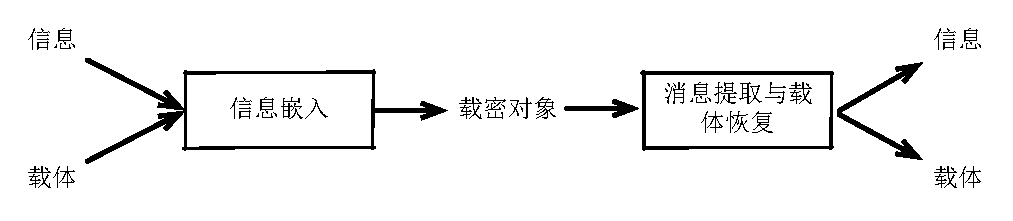
\includegraphics[width=0.8\textwidth]{figures/reversible_framework.eps}
\caption{可逆信息隐藏的一般框架}
\label{fig:revers_framework}
\end{figure}

\vspace{-8mm}
\begin{itemize}
  \vspace{-2.5mm}
  \item \textbf{以载体类型分类}\\
  \vspace{-9mm}
  \begin{itemize}
    \item[*] \textbf{基于空域图像}\\
    基于空域图像的可逆隐藏算法得到的大量的研究,大多数算法都以8比特灰度图像为载
    体,对像素进行一定的修改,以达到可逆隐藏的目的。本质来说,针对空域图像的可逆
    隐藏算法同可逆压缩算法类似,都需要找到像素间的相关性,通过一定的手法可逆地去
    除这些相关性,利用这些去除的冗余空间来嵌入秘密信息。同时,不同的算法在不同的
    嵌入率下有着不同的表现,有的算法针对小嵌入率进行特殊的改进,以最大限度的提高
    图像质量;而有的算法则注重嵌入容量,期望在可以容忍的图像质量下尽可能提高嵌入
    率。
    \par
    \vspace{-2.5mm}
    \item[*] \textbf{基于JPEG图像}\\
    JPEG作为当今最为流行的图像压缩算法,在可逆隐藏中也同样得到了深入关注。JPEG压
    缩基于DCT变换,而针对JPEG图像的可逆压缩算法也主要集中在对DCT变换系数,量化表
    等方面。本质上,DCT变换也是一种去除图像块冗余的算法,因此JPEG图像天然地使用
    于做可逆隐藏。一种常见的算法是利用每个图像块DCT系数中的0系数,例如可以寻找特
    殊的全零模式,因此这样的每个‘0’模式都可以被用来嵌入1比特信息。
    \par
    \vspace{-2.5mm}
    \item[*] \textbf{基于其他载体}\\
    随着可逆隐藏技术的不断发展,学者们不在将眼光局限在图像领域,他们尝试将可逆隐
    藏算法应用到更广泛的载体中。例如一些一维信号如音频\cite{shiu2014reversible}
    \cite{chen2013reversible}、心电图\cite{ibaida2013wavelet}\cite{rubio2013secure}。
    还有一些文献则将可逆隐藏的思想应用到了视频领域\cite{xu2014improved},提出了
    针对H.264视频的视频容错编码方法。文献将可逆隐藏技术同冗余片进行结合,能很有
    效的保障移动通信中的视频质量。\\
  \end{itemize}
  \vspace{-12mm}
  \item \textbf{以稳健性分类}\\
  \vspace{-9mm}
  \begin{itemize}
    \item[*] \textbf{脆弱水印}\\
    所谓脆弱水印,是一种当载体遭到修改后很容易被改变或毁掉的印记。由此可见,脆弱
    水印并不适合进行版权保护等工作,因为攻击者很容易就可以破坏载体中的水印。然而
    正是脆弱水印的这种对修改的敏感性,使得其被广泛的应用于图像鉴别、图像完整性认
    证等应用中。而同签名技术相比,脆弱水印也存在一定的优势,那就是它被嵌入到了载
    体中而不需要任何的附加信息,节省了通信成本。另一方面,脆弱水印能够更加精确地
    定位篡改位置,从而使得重传成本进一步降低。
    \par
    \vspace{-2.5mm}
    \item[*] \textbf{稳健水印}\\
    同脆弱水印对修改的敏感性不同,稳健水印要求载体中的水印信息在载体遭到一定的攻
    击(如压缩、加噪、滤波)时,仍然不能收到破坏,能够被提取出来完成认证工作。稳
    健水印的这种特性可以被用来进行版权认证等工作。另外,稳健水印的一些特性可以用
    在隐写等隐蔽通信的应用中。例如利用一些水印的抗打印、抗拍照等特性,可以将秘密
    信息隐藏到照片中,利用照片传递来进行秘密通信。\\
  \end{itemize}
\end{itemize}



\section{本文研究内容及工作}
\label{s:contribution_of_this_thesis}
如前所述,当前信息隐藏研究重点主要集中在灰度图像上,不论是狭义上的隐写技术,还
是可逆隐藏技术,针对灰度图像的算法在过去得到了广泛的研究。可逆隐藏方面,学者们
提出了诸如基于可逆压缩的算法\cite{fridrich2001invertible}\cite{fridrich1900lossless}
\cite{celik2005lossless}、基于直方图平移\cite{ni2006reversible}
\cite{lee2006reversiblee}\cite{li2013general}、差值扩展\cite{tian2003reversible}
\cite{alattar2003reversible}\cite{alattar2004reversible}\cite{alattar2004reversible}、
预测误差扩展的算法\cite{thodi2007expansion}\cite{fallahpour2008reversible},基于
整数变换的算法\cite{coltuc2007very}\cite{chen2010reversible}\cite{wang2010efficient}
\cite{peng2012adaptive},以及能够较大程度上提升可逆隐藏效果的排序技术
\cite{kamstra2005reversible}\cite{sachnev2009reversible}\cite{li2013high}。然而
在现实生活中,使用最多的却是彩色图像,因此,可逆隐藏今后的研究领域应
该是集中在彩色图像上。
\par
由于彩色图像的R、G、B三个通道可以分别看成是三幅灰度图像,因此一般来说,传统灰度
图像的可逆隐藏算法可以分别应用到彩色图像的三个通道,做到对彩色图像的可逆隐藏。然
而这种做法并没有利用到彩色图像本身的特点,即彩色图像三个通道之间的高度相关性。
\par
本论文中提出了一种简单的基于彩色图像通道相关性的可逆隐藏算法。通过实验发现,彩
色图像的三个通道虽然像素值不同,但是它们都有相同的结构,当通过通道内的预测去除
通道内相关性之后,可以看到三个通道的预测误差的大小和结构基本相同。据此,论文里
提出了采用通道间进行二阶预测的算法。另外,基于该预测,论文提出了一种新的排序算
法:由于预测误差符合拉普拉斯分布,因此利用邻域四个像素的差值和方差,来对预测误
差的拉普拉斯分布的参数进行预测。利用论文提出的算法,彩色图像的可逆隐藏算法的嵌
入容量和图像质量得到了一定程度的提升。\\



\section{论文结构}
\label{s:thesis_structure}
本本科毕业论文一共分为四章,各章的内容如下:
\par
第一章主要介绍论文的研究背景,简单介绍了信息隐藏技术,对可逆隐藏技术进行了分类,
并简单介绍了隐写技术、可逆信息隐藏技术的分类和应用,简单陈述了论文的主要内容和
论文结构。
\par
第二章对主流的针对灰度空域图像的常用可逆隐藏算法,以及算法中常用的排序技术进行
了详细的介绍,算法包括基于可逆隐藏的算法,基于直方图平移、差值扩展、预测误差扩
展的算法,基于整数变换的算法等,最后则介绍了一种最新的针对彩色图像的可逆隐藏算
法。
\par
第三章则详细介绍分析了本论文提出的基于彩色图像通道相关性的算法。本章主要从预测
算法、排序算法、完整的嵌入算法及流程图以及实验结果四个角度对算法进行详细的展示。
\par
第四章将对本文的工作做出一定的总结,分析现有工作的不足之处,并对可能的后续工作
进行了展望。\\
